\section{Route Designer Web Page}
\label{sec:sprint1-web}

For this sprint, a route designer web page was desired. Its functionality should include a map where users could create and modify routes, as well as a user login system to restrict access to a user's own routes.

\subsection{Graphical User Interface}
\label{sub:sprint1-web-gui}

A simple user interface was designed. An initial mock-up can be seen in \autoref{fig:sprint1-web-ui}, which shows the desired layout of the route planner display. The general philosophy was to keep the layout consistent on all pages. As such, the title and the menu will be at the same position on all views, though the menu options will change depending on the permissions of the user, in this case whether the user is logged in or not.

\begin{figure}[ht]
 \caption{Web UI Mock up}
 \label{fig:sprint1-web-ui}
 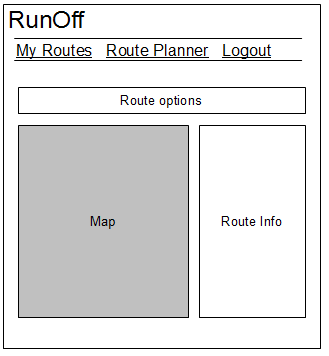
\includegraphics[scale=1]{img/webmockup1.png}
\end{figure}

Four views, which should constitute an \ac{MVP}, were planned for this sprint:
\begin{itemize}
 \item {Route Designer} (Only available when logged in)
 \item {Route Overview} (Only available when logged in)
 \item {User Registration}
 \item {User Log In}
\end{itemize}

The route overview should be a simple listing of the routes the current user has created, with a summary of the information available for that route, as well as a link to modify each route. The registration and log in views should be simple \ac{HTML} forms.

The route planner is where most of the work should be done. The planner should display a map, and the following controls on the map:

\begin{itemize}
 \item Clicking the map should add a waypoint
 \item Clicking and dragging a waypoint should move it
 \item Right-clicking a waypoint should delete it
\end{itemize}

After each of these actions has been performed, a route should be created, snapping the route to paths and pavements, as well as allowing users to see useful information, such as the total distance and topography of the route.

Additionally, the planner should expose various controls separate from the map itself, including the ability to name the route, mark it as a round-trip (Using the first waypoint as both start and end of the route) as well as submitting the route and saving it on the server.

\subsection{Database Model}

The route planner needed a database to store the routes for each user. The database design can be seen in \autoref{fig:sprint1-db-model}. This simple design allows for multiple users to store a number of routes which each have several waypoints. The index column in the \texttt{Waypoint} table is the waypoint ``number'' within the route, and this design allows sorting the waypoints correctly already at the time where they are retrieved from the database.

\begin{figure}[ht]
 \caption{Sprint 1 Database Model}
 \label{fig:sprint1-db-model}
 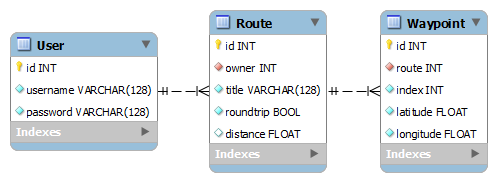
\includegraphics[scale=0.5]{img/sprint1db.png}
\end{figure}

The decision to use a boolean on the \texttt{Route} to denote whether or not the route is a round-trip, rather than saving two copies of the first waypoint with different index values, was made partly because it results ion less database entries, but the primary reason was that it made it easier to correctly load the settings of a previously saved route, should the user desire to edit it. Distance is allowed to be \texttt{null} for a route, for the reason that a user might save a route with less than two waypoints, or waypoints which might not be reachable from each other with the intent to fix it later.

\subsection{Implementation}

Implementing the web page was done in two parts, the server and client.

\subsubsection{Server Implementation}

The server was implemented in Django\cite{djangoproject}, a web framework for the Python programming language. We made use of several of the features of Django, to ease the implementation of the previously mentioned design. An example of this, is Django's \ac{ORM}, which was used to implement the database, removing any need to write database code directly. As such, the \texttt{Route} table seen in \autoref{fig:sprint1-db-model} was implemented as a Django model with the code seen in \autoref{lst:sprint1-route-model}. From this code, Django is able to generate code for several different database engines, chosen simply by changing the django settings file.

\begin{lstlisting}[language=Python,label={lst:sprint1-route-model},caption={Sprint 1 "Route" Model}]
from django.db import models
from django.contrib.auth.models import User

class Route(models.Model):
	owner = models.ForeignKey(User)
	title = models.CharField(max_length = 128)
	roundtrip = models.BoolenField(default = False)
	distance = models.FloatField(null = True)
\end{lstlisting}

The server logic implemented in this sprint is all related to insertion and retrieval of data form the database.

Another feature of Django that was used extensively is the Django Template Language. This language consists of a series of tags which can be used in \ac{HTML} pages, but are evaluated on the server before the pages are sent to the user. This introduces features such as inheritance, conditional logic and loops to \ac{HTML} pages. These features were used to ease the implementation of some of the details mentioned in \autoref{sub:sprint1-web-gui}. For example, the overall layout is written in a singe html file called \texttt{master.html}, from which each other page inherits. The master file includes a block which all of the subpages are able to overwrite with the specific content of that page. Additionally, blocks were included in the master file for page specific javascript and \ac{CSS} should it be needed.

Apart from inheritance, conditional logic were used in the templates to decide whether the logged-in or the logged-out menu should be displayed when a page is loaded, and loops were used for displaying information about a users routes in their route overview.

In this sprint, the server logic was kept quite simple, so validation features, such as having the server calculate the distance of a users routes, were not implemented, so the server simply trusts that the client does not try to submit forged information.

\subsubsection{Client Implementation}

The primary feature of the client was the route planner. This was implemented as a javascript class and makes use of the Google Maps \ac{API}\cite{gmapsapi}. The class, \texttt{Planner} is initialized with a constructor taking five arguments. Three of these should be IDs of \ac{HTML} elements which will be used to contain the map, the map options and the route information respectively. Using parameters for this allows programmers to change the layout of the route editor simply by editing the \ac{HTML} instead of the class, and keeps design and logic separate. The last two parameters for \texttt{Planner}'s constructor is the dimensions of the map, and an optional route (encoded as \ac{JSON}) to load on the map initially.

After initialization, the \texttt{Planner} instance contains a few member variables, including an array to store markers on the map and the map itself, and exposes a number of functions. Each function is described in the list below, and an overall flow of the code can be seen in \autoref{fig:sprint1-web-flow}
\begin{itemize}
 \item \texttt{initialize\_map(target)}. This function is called automatically upon construction, and sets up the map in the target \ac{HTML} element. If available, it will ask the user for permission to use geolocation\cite{geolocation} to center the map on the user's current location.
 \item \texttt{map\_events()}. This function is also called upon initialization, but after \texttt{initialize\_map} is done. This function sets up the various click events on the map.
 \item \texttt{initialize\_controls(target)}. Like \texttt{initialize\_map} this function is called upon construction, but as the name suggests, sets up the controls. This consists of generating an \ac{HTML} form for submitting the map, and inputs for naming the map, reversing order of waypoints, clearing the map and toggling whether the map is a round trip.
 \item \texttt{clear()}. This function removes any markers and directions from the map, as well as emptying the \texttt{Planner} instance's waypoint array.
 \item \texttt{update\_route()}. This function basically has two modes. The first, if the \texttt{Planner} instance has fewer than two waypoints in its array, removes rendered directions from the map. If there are more than two waypoints, it initializes a call to the Google Maps Directions service, to get directions for the route. The directions service needs to receive the waypoints in a very specific way, the code for which can be seen in \autoref{lst:update-route-1}.
 \begin{lstlisting}[label={lst:update-route-1},caption={Converting a List of Waypoints for Directions}]
var plan = []
// Extract positions. This has the nice side effect of copying the array, so markers are unaffected later on.
for (var i = 0; i < this.markers.length; i++)
{
	plan.push(this.markers[i].getPosition());
}

// If we are round-tripping, end at the last waypoint
if (this.round_trip)
	plan.push(plan[0]);

// Extract start and end point
var destination = plan.reverse().shift();
var origin = plan.reverse().shift();

// Plan now contains intermediate waypoints. Wrap these so google maps understands them
for (var i = 0; i < plan.length; i++)
{
	// Using stopover true, because it changes route algorithm to allow turning around on the spot
	plan[i] = {'location': plan[i], 'stopover': true};
}
		
var route_options = {'origin': origin,
					 'destination': destination,
					 'waypoints': plan,
					 ...}
 \end{lstlisting}
 \item \texttt{add\_marker(position, suppress\_direction)}. This function contains a bit of logic. First it checks if the number of waypoints already on the map is below the maximum allowed by the Google Maps Directions Service. If more markers can be added, it converts the \texttt{position} parameter from screen coordinates into latitude and longitude on the map, and creates the marker. It then sets up two events on the marker: One to remove the marker and call \texttt{update\_route} when the marker is right-clicked, and one to simply call \texttt{update\_route} when the marker is dragged. Finally, the \texttt{add\_marker} function itself calls \texttt{update\_route}, unless the parameter \texttt{supress\_directions} is set to true.
 \item \texttt{load(json)}. This function loads an existing route, encoded in \ac{JSON}. If the load parameter is given to the constructor, this function is called on construction, but can otherwise be called at any time. The function starts by calling \texttt{clear}. After that, it updates the controls, setting the title and round trip settings to those from the desired route. It then adds each waypoint, using the \texttt{add\_marker} function with \texttt{supress\_directions} set to true, so that the directions service is not invoked for each waypoint. Finally, it calls \texttt{update\_route}.
 \item{update\_info}. This function is called every time \texttt{update\_route} has finished. Update info does two things: First it updates the info window with the total route distance, and second it encodes the route waypoints as \ac{JSON} and stores them in a hidden field in the controls form, so that it is correclty submitted when the user submits the form.
\end{itemize}

\begin{figure}[ht]
 \caption{Sprint 1 Planner Flowchart}
 \label{fig:sprint1-web-flow}
 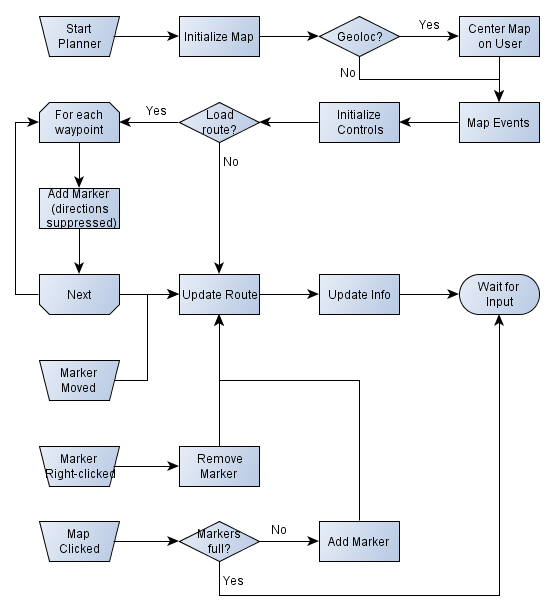
\includegraphics[width=\textwidth]{img/sprint1webflow.png}
\end{figure}


All in all, most of the functionality revolves around sending and retrieving data to and from the Google Maps \ac{API}, as well as ensuring that using the planner is as smooth as possible. The look of the planner at the end of the first sprint can be seen in \autoref{fig:sprint1-web-screen}.

\begin{figure}[ht]
 \caption{Sprint 1 Webpage}
 \label{fig:sprint1-web-screen}
 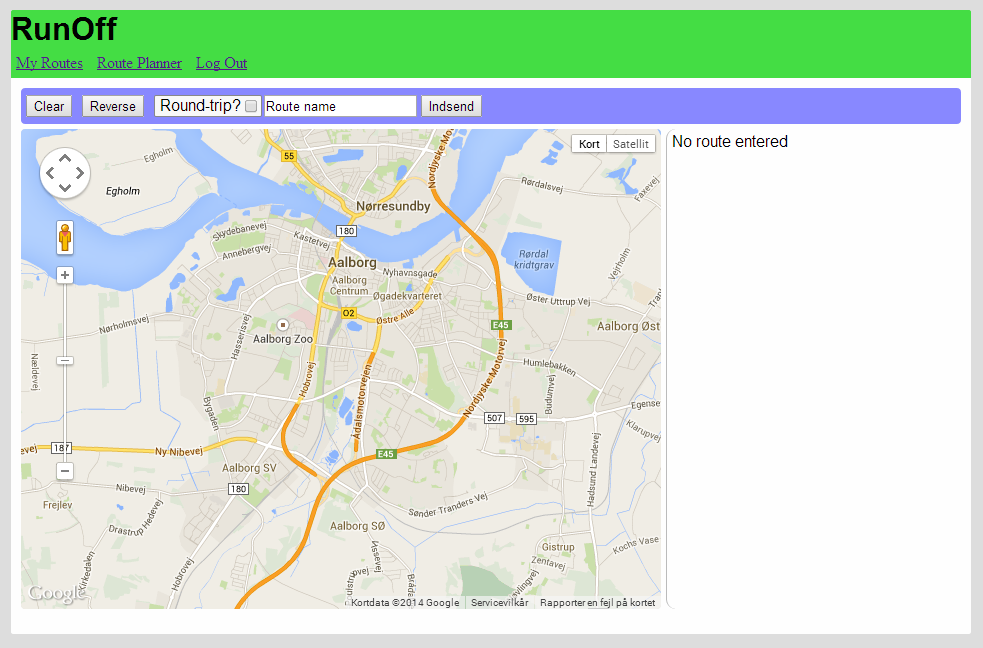
\includegraphics[width=\textwidth]{img/webplanner1.png}
\end{figure}

\subsection{Tests}

The testing effort for the web page in this sprint revolved mostly around the \texttt{Planner} javascript class. A unit test suite was set up using the QUnit testing library\cite{qunit}, including 25 assertions across 8 different tests, attempting both legal and illegal operations. The Blanket coverage tool\cite{blanketjs} reports the unit tests to have 81\% code coverage.

Additionally, informal testing was accomplished by having each member of the group use the route planner.
